\section{Data and Measurement}\label{sec:data}

The starting panel is the repository's frozen merge of the Digital Society
Project (DSP) v8, World Development Indicators (WDI), and Worldwide Governance
Indicators (WGI). It contains 4,539 country-years for 175 countries in
2000--2025. DSP v8 itself covers 179 countries over those years
\citep{mechkova2026dsp}; this coverage does not imply that every regression
contains 175 countries. Observed outcomes and horizon-specific sample sizes
are reported below and in the generated tables.

\subsection{What the index measures}\label{subsec:index}
DSP combines expert assessments through a measurement model
\citep{pemstein2018latent}. The five components concern false-information
dissemination by governments domestically and abroad, political parties
domestically and abroad, and foreign governments into the country. Each
component is reversed so that higher values indicate more disinformation,
then standardized. Weights are respectively $(1/4,1/8,1/4,1/8,1/4)$ in that
ordering. The weighted composite is transformed into its pooled percentile,
using $(\mathrm{rank}-1/2)/n$ with average ranks for ties. The resulting
$M_{r,t}$ lies strictly between zero and one.

These are indicators of the broad political information environment. They
are not financial-content counts, measured exposure, belief adoption or
financial-message accuracy. A value of $0.89$ means approximately the 89th
percentile of the reference distribution; it does not mean that 89 percent
of financial messages are false. No financial-specific validation sample is
available in this replication package. Domestic-only or equal weights probe
index construction but cannot supply that missing construct validity.
The haircut mechanism in Section~\ref{sec:model} therefore motivates a
hypothesis rather than a measured channel.

The retrospective regressions retain the pooled transformation for
comparability. Raw-composite and alternative-weight estimates are reported,
rather than assuming that slopes are invariant to monotone transformations.
For forecasting, component means, standard deviations and the empirical CDF
are re-estimated using each training window only. Evaluation observations
outside the training range are clipped to its finite endpoint ranks. The
DSP component data required for this procedure are included in the
replication data, with source and checksum records.

\begin{figure}[!htbp]\centering
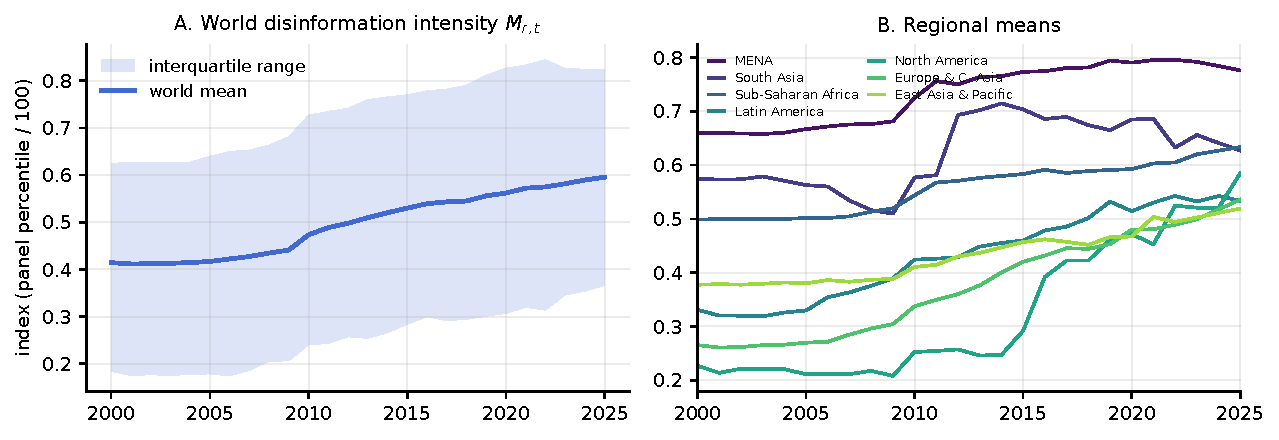
\includegraphics[width=\linewidth]{figures/fig1_index_trends.pdf}
\caption{The retrospective disinformation index. The world mean, interquartile
range and regional means describe relative positions in a pooled distribution,
not estimated shares of false financial messages.}\label{fig:index}
\end{figure}

\subsection{Outcomes and conditioning variables}\label{subsec:outcomes}
Real GDP, gross fixed capital formation and export growth are WDI annual
percentage changes \citep{worldbank2026wdi}. Capital formation is labeled
\emph{investment}; it does not specifically identify innovation finance.
Gini and nonperforming-loan (NPL) ratios provide distributional and banking
outcomes. These outcome series are never interpolated or filled in the
estimation. Growth outcomes sum observed annual rates from $t$ to $t+h$;
this is a cumulative percentage-point sum, not compounded GDP-level growth.
Gini and NPL outcomes are observed endpoint changes from $t-1$ to $t+h$.

Conditioning states are NPLs, trade openness and inequality. Missing NPL
conditioning values may use the previous observation for at most two years;
Gini conditioning values may use it for at most five years. No future
observation is used to fill these states, and a no-fill specification is
reported separately. The frozen input includes two-sided interpolated columns
for provenance; they are replaced in memory before estimation. Calendar-year
matching prevents a gap from being mistaken for a one-year lag.

Controls include lagged GDP growth, log real GDP per capita, CPI inflation
clipped to $[-10,60]$, and government effectiveness. Investment and export equations also
include the lagged observed outcome; lagged NPL and Gini levels already enter
as conditioning states. The frozen WGI vintage ends in 2022 and
its existing forward-carried values are retained through 2025; an end-2022
sample check is reported. Historical source releases and contemporaneous
publication dates are not reconstructed, so the forecasting exercise uses
latest-vintage data and cannot be described as real-time validation.

\input{tables/summary_table}
